\chapter{Expérimentations}
\label{chap:implementation}

Dans ce chapitre, nous allons présenter des expérimentations visant à appliquer à des cas d'usage concrets les méthodes présentées dans les chapitres précédents.

% 1. Cas d'usage: je veux produire quelque chose
% 2. J'utilise les chapitres 2 et 3 pour générer ce que je veux générer

% \section{QGIS2Desc: Un plugin QGIS pour personnaliser la description}

% % Transcription: 6 mn

% Dans le chapitre \ref{chap:description}, nous avons présenté un cadre permettant de réaliser une description au sein d'un SIG en partant de données géographiques. Dans cette partie, nous allons présenter son implémentation au sein du SIG QGIS. 

% \todo{}

\section{Du graphe OpenStreetMap à la description exocentrée}

\label{sec:implementation_segmentation}

Cette partie présente une expérimentation visant à décrire textuellement un carrefour depuis \gls{osm}, en concevant la description au sein d'un \gls{sig}. Elle s'appuie, pour le déroulé général, sur le cadre présenté dans le chapitre \ref{chap:description} où les rôles de définition du besoin et de conception technique sont assumés par différents profils d'utilisateurs. Elle s'appuie également sur les modélisations du carrefour présenté en chapitre \ref{chap:modelisation} pour l'acquisition des données.

\subsection{Conception du canevas modulaire}

À l'instar de ce que nous avons présenté au sein du chapitre précédent, la conception du canevas modulaire doit être prise en charge par l'utilisateur final de l'outil. Il doit ainsi préparer la forme des textes souhaités, la forme des données nécessaires, et définir sur cette base les patrons textuels à implémenter (\ref{fig:desc_canevas_modulaire}). Dans le cas de la description de carrefours, cette étape est assumée par l'\gls{ia}, en collaboration avec la ou les personnes qu'il accompagne pour définir des descriptions adaptées à leur besoin.

\subsubsection{Préparation du texte}

Le texte préparé pour cette expérimentation est issu d'échanges avec des personnes liées à la déficience visuelle, notamment des personnes concernées, des \gls{ia}, des architectes urbains et des entreprises de mobilité. L'objectif est ici d'obtenir un aperçu synthétique de la configuration du carrefour: sa forme, ses branches et les manières de le traverser. Pour décrire la forme du carrefour, bien que non-normalisé, un consensus à la fois mobilisés par les urbanistes et usagers existe autour des appelations <<~en croix~>>, <<~en T~>>, etc \cite{fogliaroni2018}, qui donne à la fois une information sur le nombre de branches et sur la forme générale du carrefour. Pour chaque branche, on détermine le nombre de voies, le type de véhicule qui circule dessus, et les sens de circulation. Enfin, on détermine pour chaque branche s'il existe une traversée, c'est-à-dire la possibilité de passer d'un trottoir à l'autre, et on décrit l'accessibilité des passages piéton qui y sont associés. Par ailleurs, toutes les descriptions ont lieu dans le sens de sens des aiguilles d'une montre en partant de la branche la plus au nord. Le plan de la description est présenté sur la figure \ref{fig:experimentation_plan_description}.

\begin{figure}[ht]
    \begin{minipage}[b]{0.45\linewidth}
        \centering
        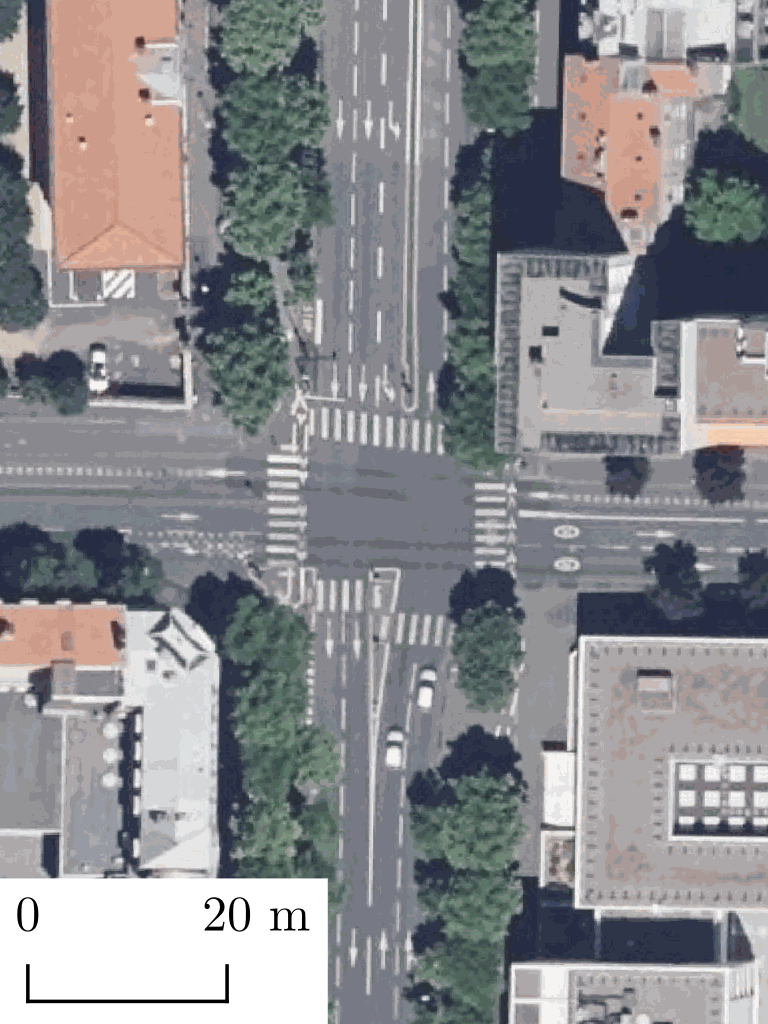
\includegraphics[width=0.8\linewidth]{images/experimentation/ortho_carrefour.png} 
    \end{minipage}
    \begin{minipage}[b]{0.45\linewidth}
        \footnotesize
        \textbf{Description générale}\\
        Le carrefour à l'intersection du cours Sablon et de l'avenue Carnot est un carrefour à 4 branches.\\
        \textbf{Description des branches}\\
        (...)\\
        La branche numéro deux qui s'appelle avenue Carnot est composée d'une voie de bus sortante, et une voie de circulation et une voie de bus entrante.\\
        (...)\\
        \textbf{Description des traversées}\\
        (...)\\
        La branche numéro trois se traverse en trois fois. Les passages piétons ne sont pas tous protégés par un feu. Il manque des bandes d'éveil de vigilance ou celles-ci sont dégradées.\\
        (...)
    \end{minipage}
    \caption{Exemple de description souhaitée pour un carrefour en croix en suivant le plan établi. Source: IGN BD Ortho 2020.}
    \label{fig:experimentation_plan_description}
\end{figure}

\subsubsection{Préparation de la forme des données}

\label{sec:experimentation_forme_donnees}

Pour générer le texte préparé, il faut disposer des données nécessaires à la description du carrefour. La conception du plan est divisée en trois parties pouvant chacune représenter une donnée:

\newpar{}

\textbf{La description générale} présente une vue synthétique du carrefour: nom des branches et type de carrefour. Une difficulté réside dans la variabilité du nombre de branches et de leur nom. Nous avons décidé ici de stocker les noms de branche au sein d'un unique champ dans le format JSON. La donnée peut alors suivre le schéma tabulaire défini en table \ref{tab:experimentation_desc_generale}.

\newpar{}

\begin{table}[ht]
    \begin{center}
        \footnotesize
        \begin{tabular}{ | l | l |}
            \textbf{Nombre branche} & \textbf{Noms branches}\\
            \hline
            4 & 
            \makecell{
                \texttt[\\
                \hspace{0.5cm}\texttt{\{"type": "avenue","name": "Carnot"\}},\\
                \hspace{0.5cm}\texttt{\{"type": "cours","name": "Sablon"\}}\\
                \texttt]
            }
        \end{tabular}
    \end{center}
    \caption{Le nom des branches est séparé en type et en nom afin de permettre la liaison lors de la réalisation du texte.}
    \label{tab:experimentation_desc_generale}
\end{table}

\newpar{}

\textbf{La description des branches} doit indiquer pour chaque branche son numéro et, dans le sens des aiguilles d'une montre, les voies qui le composent. À l'instar des noms de branche, le nombre de voies est également variable. Par ailleurs, il doit être possible de décrire un enchaînement de voies de types et de sens différents. À l'instar de la solution précédente, ces informations seront stockées dans une unique colonne au format JSON. On peut alors définir le schéma tabulaire en table \ref{tab:experimentation_desc_branches}.

\newpar{}

\begin{table}[ht]
    \begin{center}
        \footnotesize
        \begin{tabular}{ | l | l |}
            \textbf{N° branche} & \textbf{Voies}\\
            \hline
            2 & 
            \makecell{
                \texttt[\\
                \hspace{0.5cm}\texttt{\{"number": 1,"direction": "sortante","type": "bus"\}},\\
                \hspace{0.5cm}\texttt{\{"number": 1,"direction": "entrante","type": "car"\}}\\
                \texttt]
            }
        \end{tabular}
    \end{center}
    \caption{Le champ voie décrit l'enchainement des voies du la branche. Pour chaque couple de direction et de type, le nombre de voies contigües concernées est indiqué.}
    \label{tab:experimentation_desc_branches}
\end{table}

\newpar{}

\textbf{La description des traversées} affiche une vue synthétique par branche de la traversée quand elle est présente. On ne décrit pas chaque passage piéton mais les caractéristiques générales de la traversées: nombre de passages piétons, présence intégrale, partielle, ou nulle de feux et de pavage tactile. Le schéma tabulaire est présenté en table \ref{tab:experimentation_desc_traversées}.

\newpar{}

\begin{table}[ht]
    \begin{center}
        \footnotesize
        \begin{tabular}{ | l | l | l | l | }
            \textbf{N° branche} & \textbf{Nombre passages piéton} & \textbf{Feux piétons} & \textbf{Pavage tactile}\tabularnewline
            \hline
            3 & 2 & complet & complet
        \end{tabular}
    \end{center}
    \caption{Pour chaque branche, les caractéristiques de la traversée sont renseignées.}
    \label{tab:experimentation_desc_traversées}
\end{table}

\subsubsection{Préparation des patrons textuels}

\label{sec:experimentation_preparation_patron}

En disposant du texte final et de la forme des données, on peut maintenant définir les patrons textuels de chaque partie. Un patron textuel correspond à un texte conditionnel dont le contenu pourra varier selon les attributs de la donnée décrite. Un exemple de patron applicable à la description générale est présenté par l'algorithme \ref{alg:experimentation_patron_generale}.

\begin{algorithm}
\begin{algorithmic}
    \State $texte:=$ \texttt{"Le carrefour à l'intersection de"}
    \For{{chaque $type$, $nom$ dans $NomsBranches$}}
        \State $texte \leftarrow texte + type + nom$
    \EndFor
    \State $texte \leftarrow texte +$\texttt{"est un carrefour à"}$+ NombreBranches+$\texttt{"branches".}
\end{algorithmic}
\caption{Patron textuel de la description générale}
\label{alg:experimentation_patron_generale}
\end{algorithm}

On remarque que le patron présenté ci-dessus ne correspond pas exactement au texte souhaité. Exécuté avec les données précédentes, le texte obtenu serait "Le carrefour à l'intersection avenue Carnot cours Sablon est un carrefour à 4 branches". Il manque en effet les prépositions pour avenue et cours (<<~de l'~>> et <<~du~>>), de même qu'un "et" entre les deux noms de branche. Cet aspect est adressé dans l'implémentation présentée en partie suivante.

\subsection{Intégration du canevas dans un \gls{sig}}

L'intégration du canevas conçu par l'utilisateur est réalisée par un géomaticien ou une personne formée à l'utilisation d'un \gls{sig}. Cette intégration se fait en plusieurs étapes: il faut rechercher les données effectivement disponibles au regard des besoins exprimés, les transformer selon les formes établies par l'utilisateur, puis implémenter les patrons et la génération du texte final dans le \gls{sig}. Pour cette expérimentation, les traitements ont été réalisés sous QGIS. Des développements spécifiques en Python pour le traitement des données \gls{osm} liées au carrefour et pour la génération de texte ont été réalisé et sont présentés dans les parties suivantes.

\subsubsection{Acquisition des données}

Le texte préparé implique d'avoir accès à des données liées à la voirie à la fois des points de vue motorisé (nombre de voies) et piéton (trottoirs, passages piéton, signalisation), mais également à des informations sur l'accessibilité des équipements (\gls{bev}, signaux sonores). Comme évoqué dans le chapitre \ref{chap:etat_art}, ces informations sont accessibles au sein de bases de données éparses réalisées par les collectivités gestionnaires de la voirie et des équipements. Elles peuvent effectivement être utilisées, mais à condition de contraindre la réalisation des descriptions au territoire sur lesquelles elles sont disponibles. En revanche, les informations intrinsèques au carrefour (délimitation du carrefour et de ses branches) ne sont pas disponibles et doivent être calculées dans tous les cas. Nous avons développé des outils permettant d'obtenir ces informations à partir d'\gls{osm}.

\newpar{}

Nous avons déjà présenté les méthodes mobilisées pour délimiter un carrefour et ses branches dans la partie \ref{sec:modelisation_crseg}. Ces méthodes ont été implémentées en Python au sein d'un outil nommé crseg et publié sous la forme d'un logiciel libre\footnote{https://github.com/jmtrivial/crossroads-segmentation}, qui permet, à partir du graphe de données issu d'\gls{osm} de délimiter les carrefours et, pour chaque carrefours, séparer son cœur de ses branches. Il présente plusieurs paramètres détaillés en partie \ref{sec:modelisation_crseg} et sur la forge logicielle de l'outil. Il permet, en sortie, d'obtenir pour chaque région du carrefour (cœur du carrefour, branches, bordures) les nœuds correspondants au format JSON (voir figure \ref{fig:experimentation_crseg_json}).

\begin{figure}
    \centering
    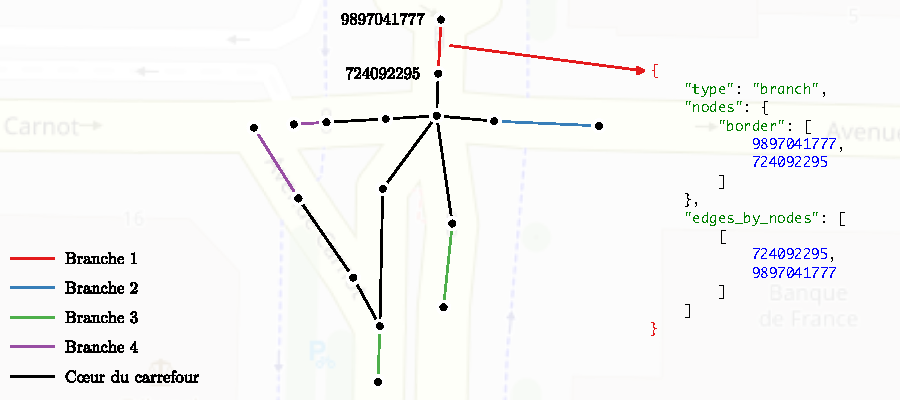
\includegraphics{images/experimentation/donnees_crseg.pdf}
    \caption{Les données obtenues par crseg permettent d'identifier les nœuds appartenant à la branche. Source: Contributeurs OpenStreetMap.}
    \label{fig:experimentation_crseg_json}
\end{figure}

\newpar{}

Faisant suite à la délimitation du carrefour, nous présentions dans la partie \ref{sec:modelisation_calcul_info_pietonnes} les méthodes permettant à partir des branches d'obtenir sur le carrefour les trottoirs, les îlots, et les traversées de branches. Ces méthodes ont également été implémentées en Python au sein d'un outil nommé crmodel et publié sous la forme d'un logiciel libre\footnote{https://github.com/jeremyk6/crmodel}. crmodel prend en entrée le même graphe de données \gls{osm} utilisé par crseg, ainsi que le JSON de segmentation produit par crseg. Un exemple de résultat calculé par crmodel est présenté en figure \ref{fig:experimentation_crmodel_info_pietonne}.

\begin{figure}
    \centering
    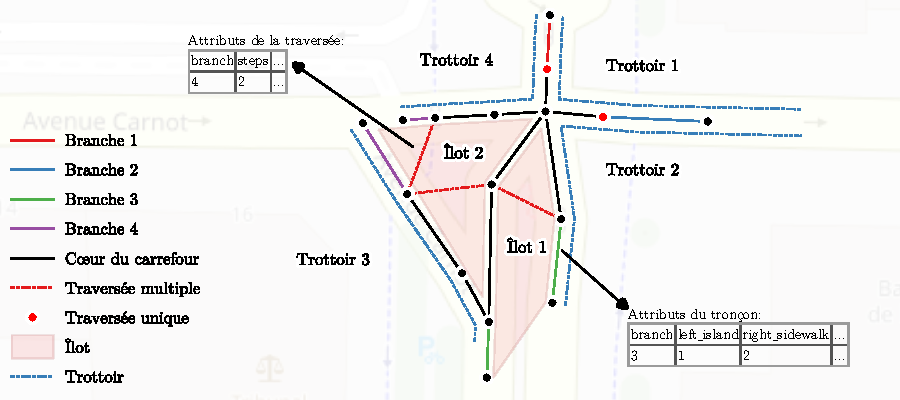
\includegraphics{images/experimentation/donnees_crmodel.pdf}
    \caption{Les informations piétonnes calculées à partir de crseg ne forment pas de nouvelle géométrie mais existent sous forme sémantique sur les tronçons originaux. Seules les traversées multiples forment de nouvelles géométries en étant composées des nœuds de passage piéton permettant de passer d'un trottoir à l'autre sur une branche. Source: Contributeurs OpenStreetMap.}
    \label{fig:experimentation_crmodel_info_pietonne}
\end{figure}

\newpar{}

crmodel comprend, au-delà de la création de ces nouvelles informations, une seconde étape: l'instanciation du modèle CrModel, présenté en partie \ref{sec:modelisation_crmodel}. Celui-ci est prévu pour représenter un carrefour et intégrer au sein d'un modèle objets tous les éléments nécessaires à sa description, facilitant la manipulation des données. En partant du modèle, l'outil permet d'exporter un format GeoJSON spécifique pouvant être intégré dans un SIG et définissant pour chaque entité le type d'objet concerné (tronçon de route, branche, passage piéton, traversée) et les attributs associés.

\newpar{}

L'outil crmodel en ligne de commande embarque crseg et permet de visualiser le résultat de la segmentation avec la commande \texttt{crmodel -c x y} (x et y correspondant à la position approximative du centre du carrefour). Celle-ci peut être ajustée à l'aide des paramètres pour obtenir un résultat satisfaisant. On peut alors ajouter \texttt{-o carrefour.geojson} pour obtenir le fichier à intégrer à QGIS. Pour faciliter son utilisation par un utilisateur final, le géomaticien peut embarquer l'outil dans un traitement graphique exposant ses paramètres.

\subsubsection{Transformation des données}

Le format GeoJSON, pratique pour proposer un export rapide de l'intégralité des entités et attributs de CrModel, n'est pas rendu par QGIS d'une manière directement exploitable pour la génération de texte. Cependant, il contient l'intégralité des informations nécessaires à la génération du format de couches établies en partie \ref{sec:experimentation_forme_donnees}. On peut alors exploiter les outils intégrés à QGIS pour transformer l'export dans le format attendu. Cette étape de transformation peut être réalisée manuellement ou intégrée à une chaîne de traitements Processing, l'outil de scripting graphique intégré à QGIS, pour automatiser toute transformation similaire ultérieure et appliquer la transformation sur d'autres territoires. La chaîne de transformation et le résultat obtenu sont illustrés en figure \ref{fig:experimentation_chaine_donnees_qgis}.

\begin{figure}[ht]
    \centering
    \begin{subfigure}[t]{.49\linewidth}
        \centering
        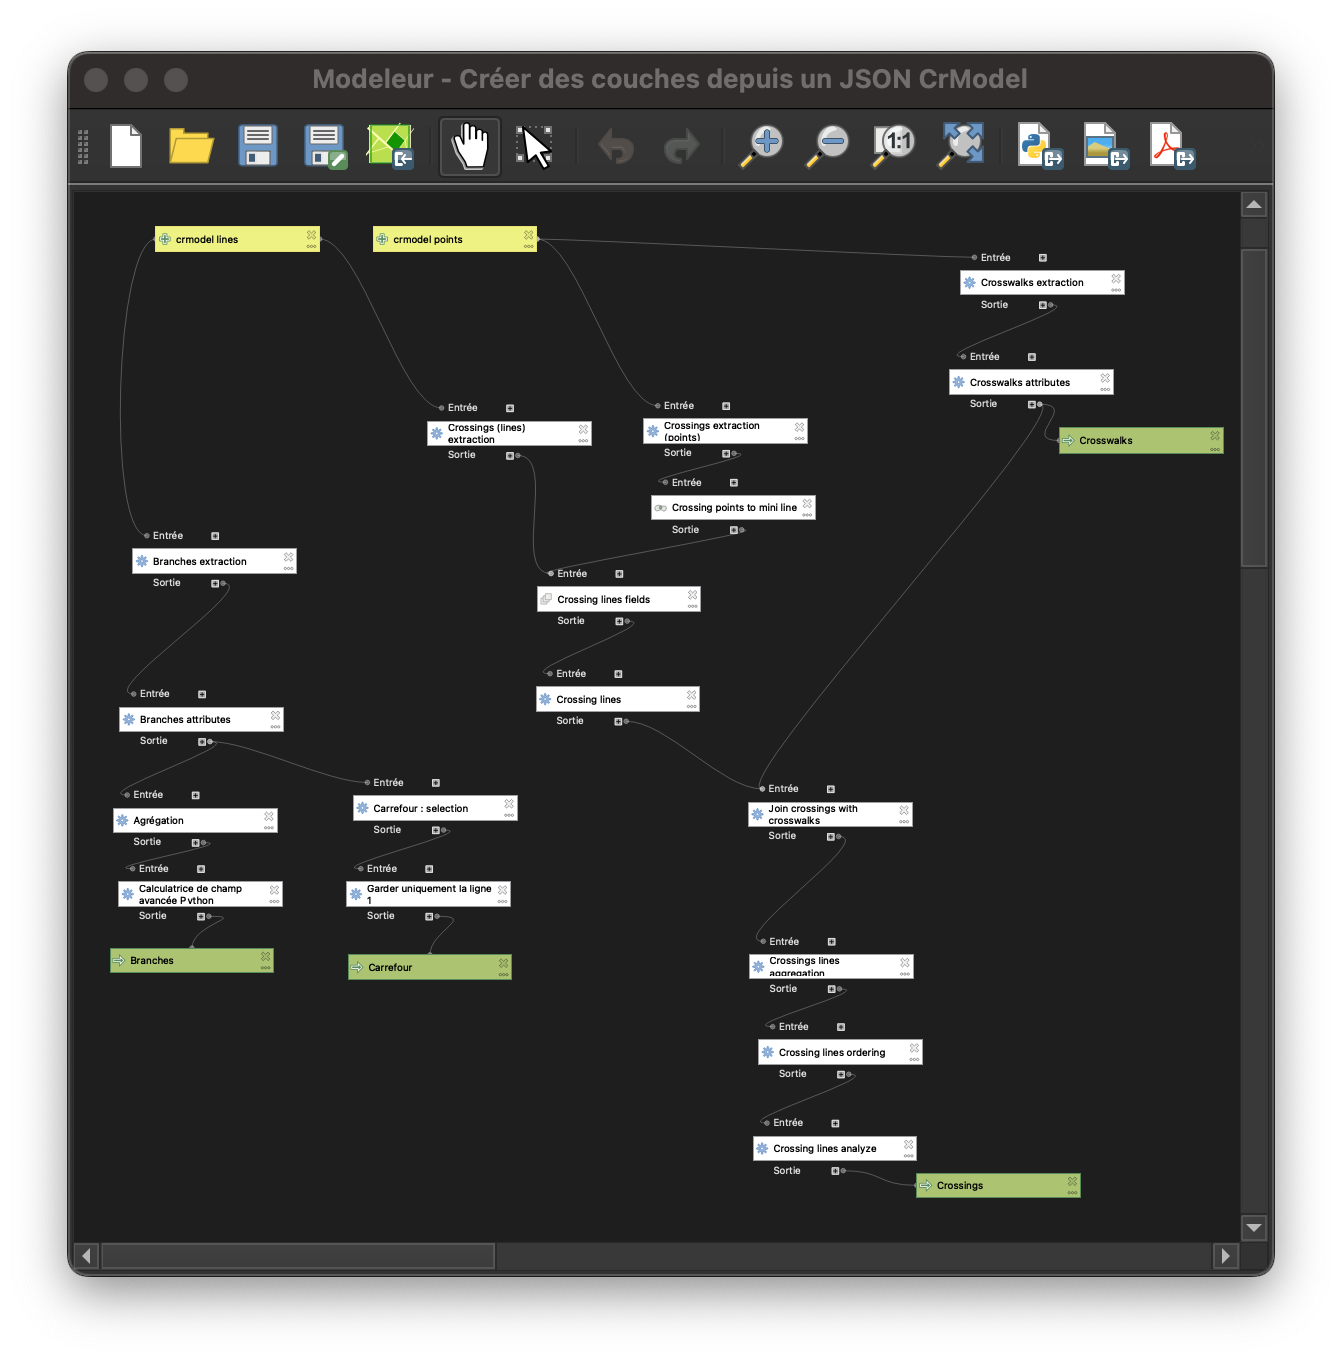
\includegraphics[width=0.8\textwidth]{images/experimentation/pipeline_processing_crmodel.png}
        \caption{Automatiser les traitements permet d'exécuter la chaîne sur de nouveaux territoires.}
        \label{fig:experimentation_transformation_qgis}
    \end{subfigure}
    \begin{subfigure}[t]{.49\linewidth}
        \centering
        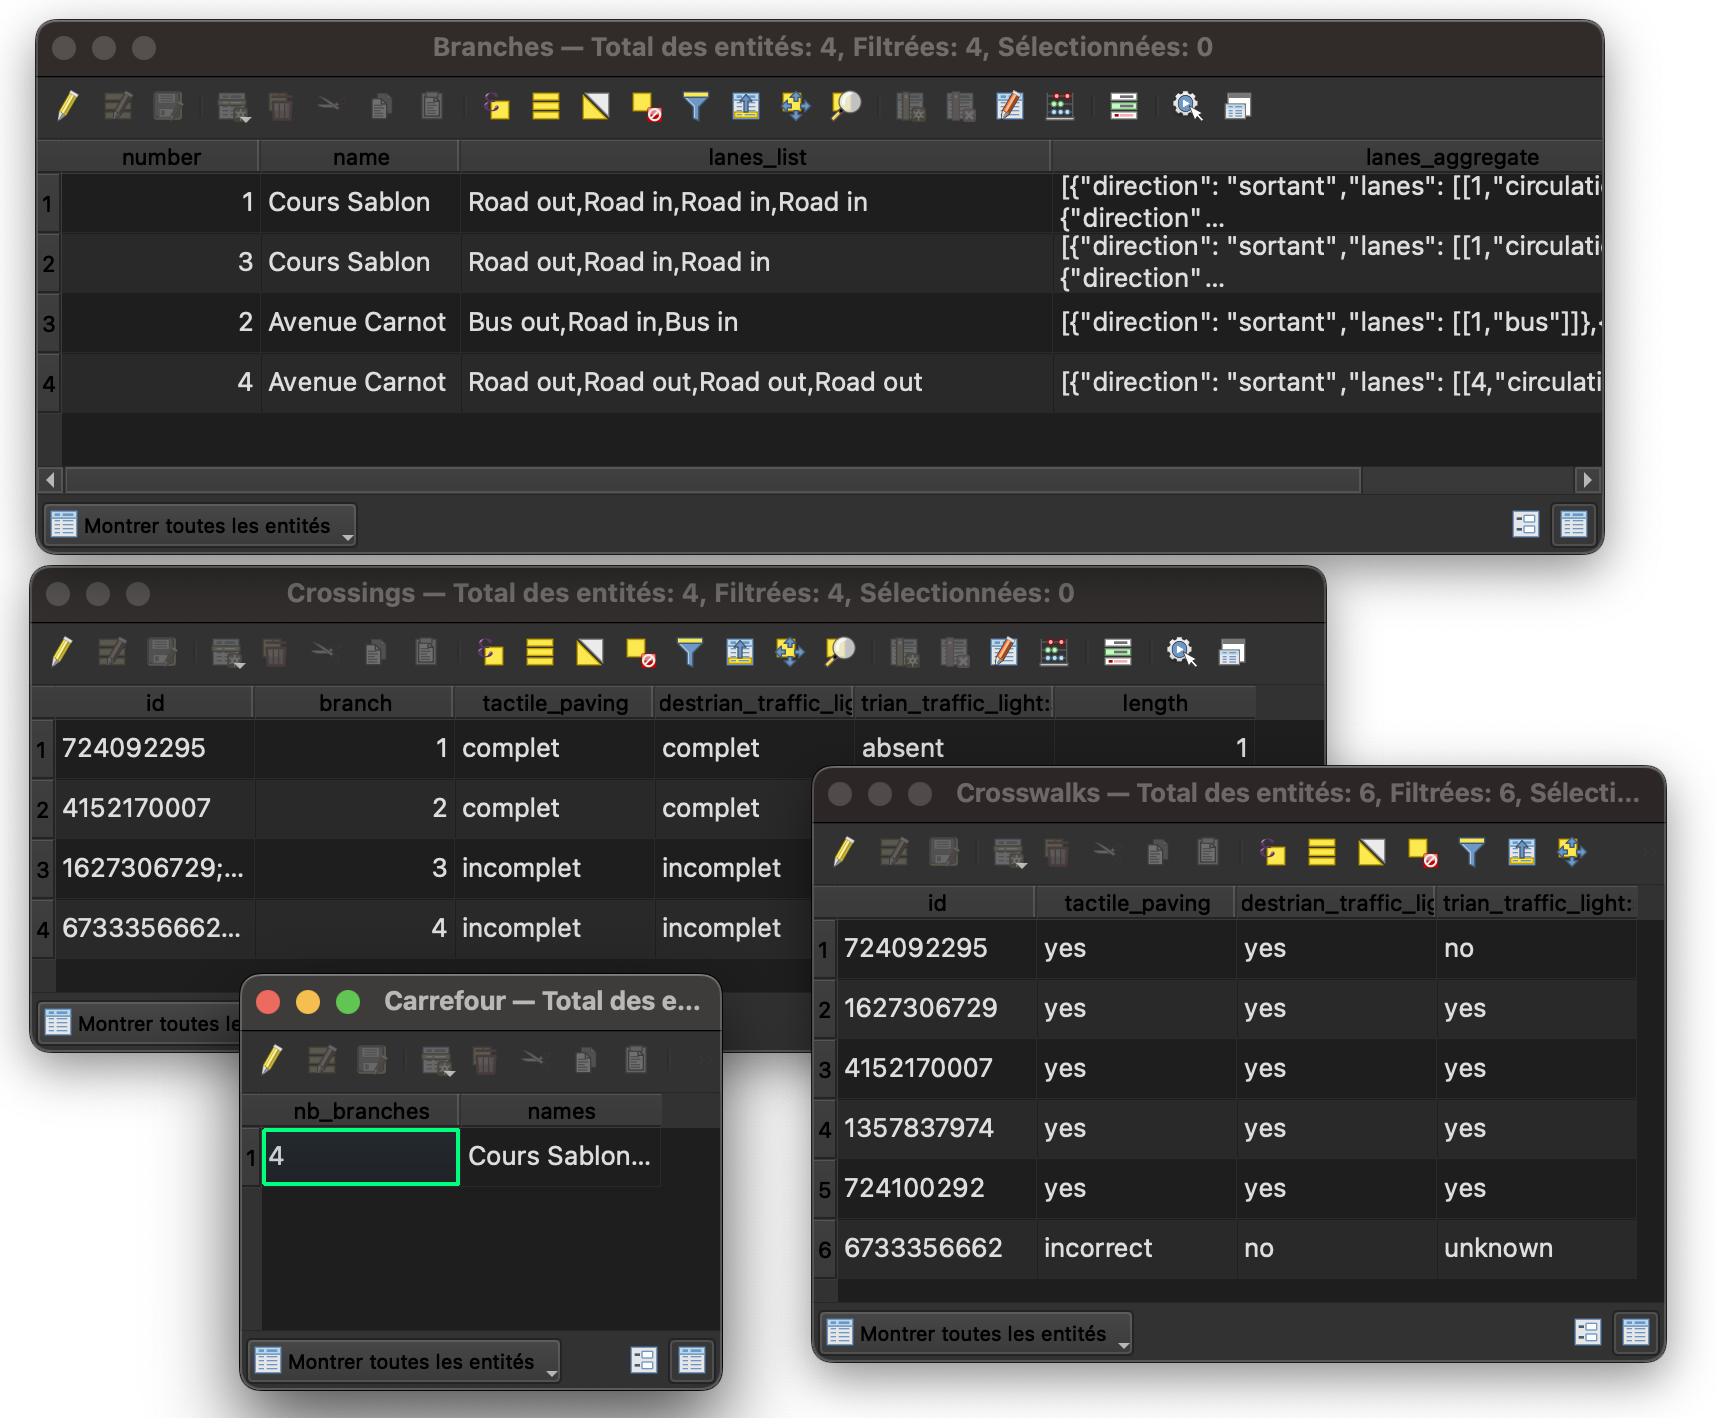
\includegraphics[width=\textwidth]{images/experimentation/resultat_processing_crmodel.png}
        \caption{Les données transformées correspondent au format établi par l'utilisateur en partie \ref{sec:experimentation_forme_donnees}.}
        \label{fig:experimentation_transformation_resultat_qgis}
    \end{subfigure}
    \caption{La chaîne de traitements de données sous QGIS permet de partir du GeoJSON fourni par crmodel pour obtenir un format exploitable pour la description.}
    \label{fig:experimentation_chaine_donnees_qgis}
\end{figure}

\subsubsection{Implémentation des patrons et de la description}

Les données adaptées à la description en notre possession, nous pouvons maintenant implémenter les patrons de description puis leur assemblage sous QGIS. Pour le permettre, nous avons implémenté une extension à QGIS nommé QGIS2Desc, qui s'intègre à Processing pour proposer deux nouveaux traitements.

\newpar{}

Le premier s'appelle "Concevoir une description" et va permettre l'implémentation d'un patron de description à partir d'une couche. Il prend en entrée une couche à décrire et offre à l'utilisateur un champ de texte permettant de définir le patron en Python. Plusieurs facilitations sont proposées, notamment en permettant l'accès simplifié aux attributs de la couche. Par ailleurs, pour répondre à la problématique des prépositions soulevées en partie \ref{sec:experimentation_preparation_patron}, il est possible d'utiliser le réalisateur de texte JSRealB \cite{molins2015} pour segmenter tout ou partie du texte en syntagmes et permettre la gestion des prépositions, des pluriels, des déterminants, des conjonctions, etc. Enfin, Il est possible d'ajouter au texte un ensemble de métadonnées qu permettrons de le sélectionner lors de l'étape d'assemblage. En sortie du traitement, la couche d'origine est complétée de deux champs supplémentaires au format JSON:

\begin{itemize}
    \item "description" contient le texte établi pour chaque ligne au format défini par JSRealB pour permettre sa réalisation ultérieure.
    \item "metadata" contient les métadonnées définie précédemment.
\end{itemize}

La figure \ref{fig:experimentation_qgis2desc_conception} est une capture d'écran qui montre l'usage du traitement pour obtenir la description générale du carrefour.

\begin{figure}[ht]
    \centering
    \resizebox{7cm}{!}{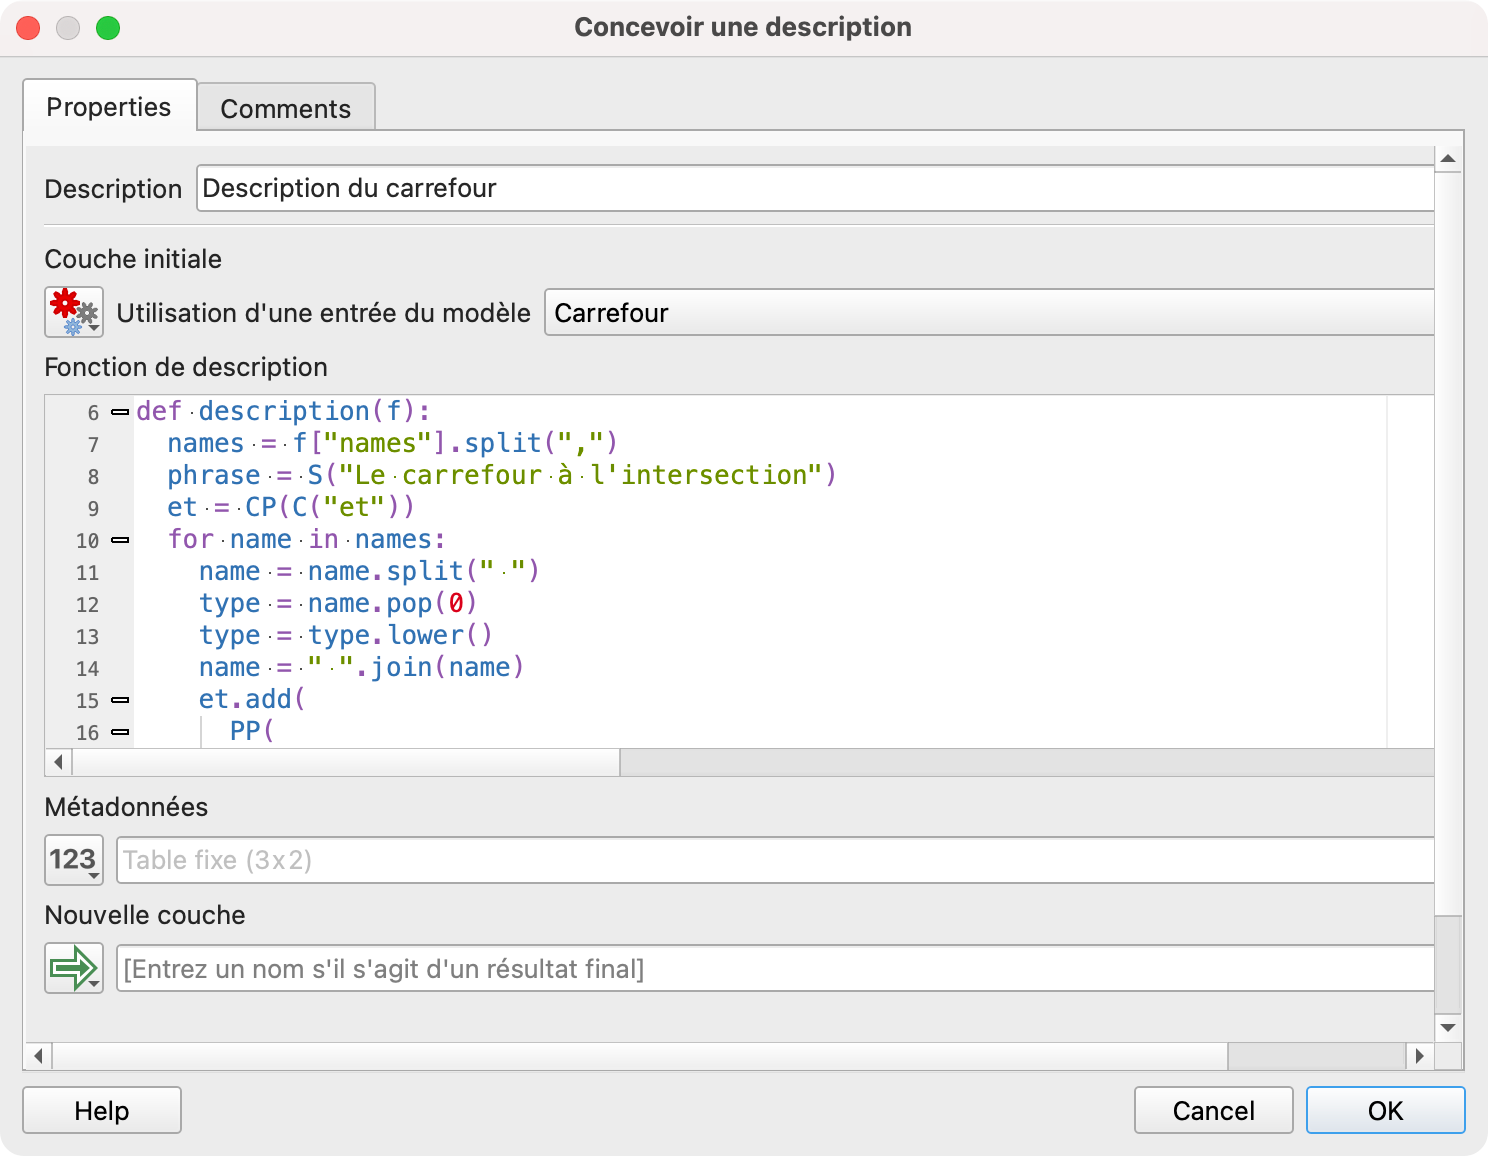
\includegraphics{images/experimentation/qgis2desc_conception.png}}
    \caption{Dans le patron, on remarque l'usage des fonctions \texttt{CP} et \texttt{C} qui vont permettre de réaliser la coordination entre les noms de branche. Pour deux branche, on obtiendra le texte "branche 1 et branche 2". Pour trois branches et plus, on obtiendra le texte "branche 1, branche 2, branche 3, (...) et branche n"}
    \label{fig:experimentation_qgis2desc_conception}
\end{figure}

\newpar{}

Le second s'appelle "Assembler des descriptions" et va permettre de générer le document final. Il prend en entrée plusieurs couches issues de "Concevoir une description", un ensemble de métadonnées correspondantes à celles définies à l'étape précédente et qui va permettre de sélectionner les descriptions à prendre en compte, et un plan de description. Le plan de description correspond à un tableau ordonné dont le format est indiqué par le tableau \ref{experimentation:table_plan_description}. Chaque entrée du tableau est prise en compte de haut en bas et définit la couche décrite, le titre de la partie, et la forme que prendra le texte (actuellement un texte brut et une liste simple ou numérotée). La figure \ref{fig:experimentation_assemblage} présente un exemple d'assemblage de la description.

\begin{table}
    \begin{center}
    \footnotesize
    \begin{tabular}{ | l | l | l | }
        Couche & Titre & Forme\tabularnewline
        \hline
        general & Description générale & text\\
        branches & Description des branches & numbered\_list\\
        crossings & Description des traversées & numbered\_list
    \end{tabular}
    \end{center}
    \caption{Le plan de la description défini précédemment serait le suivant dans le traitement établi.}
    \label{experimentation:table_plan_description}
\end{table}

\begin{figure}[ht]
    \centering
    \begin{subfigure}[t]{.49\linewidth}
        \centering
        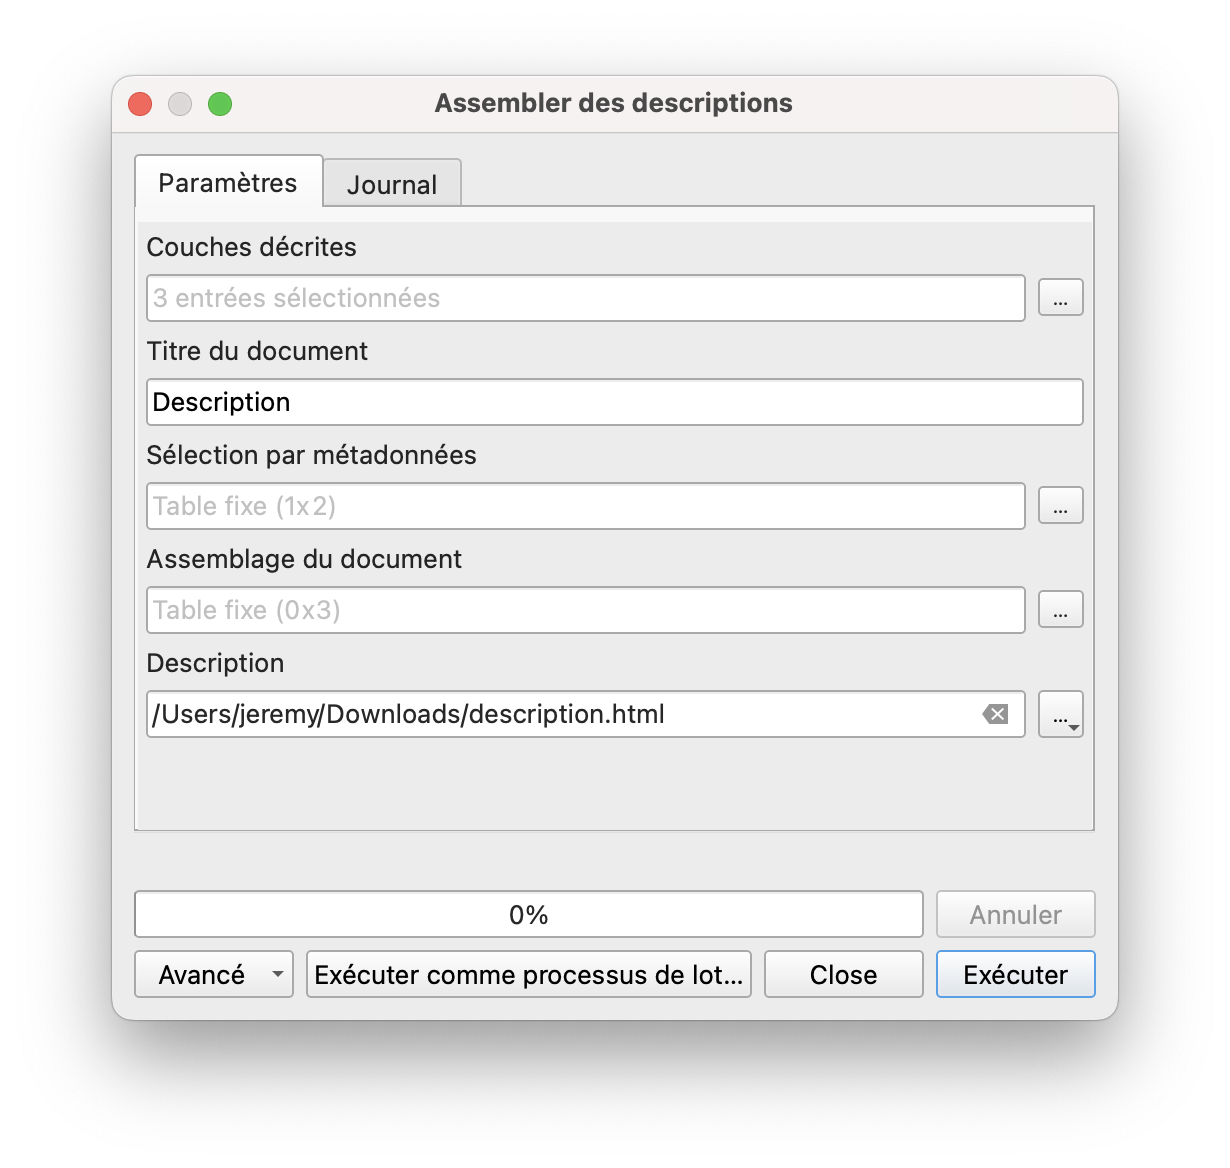
\includegraphics[width=0.6\textwidth]{images/experimentation/qgis2desc_assemblage.png}
        \caption{La fenêtre de "Assembler les descriptions" présente ses différents paramètres.}
        \label{fig:experimentation_assemblage_fenetre}
    \end{subfigure}
    \begin{subfigure}[t]{.49\linewidth}
        \centering
        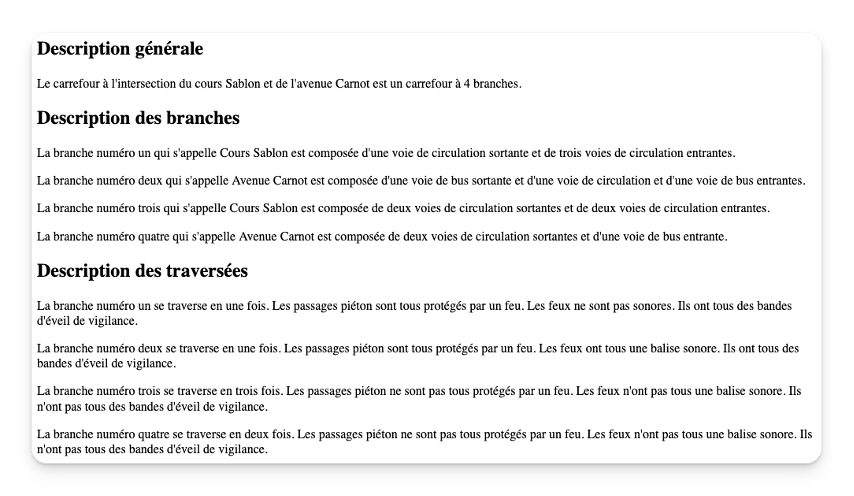
\includegraphics[width=\textwidth]{images/experimentation/qgis2desc_html.png}
        \caption{La sortie HTML obtenue respecte le formatage défini dans le plan.}
        \label{fig:experimentation_assemblage_html}
    \end{subfigure}
    \caption{Le traitement actuel permet d'obtenir en sortie un document HTML, mais son code est cependant extensible pour permettre la génération d'autres types de documents.}
    \label{fig:experimentation_assemblage}
\end{figure}

\newpar{}

À l'instar des traitements de données, il est possible d'intégrer les patrons et l'assemblage dans un traitement Processing pour permettre sa réutilisation sur de nouvelles données. Un modèle graphique Processing devient sous QGIS un traitement comme un autre avec des entrées, des sorties, et des paramètres. Il est ainsi possible d'exposer les paramètres de l'assemblage comme les métadonnées à sélectionner ou le plan de la description afin de permettre à un utilisateur final de moduler la description obtenue. La figure \ref{fig:experimentation_qgis2desc_modele_assemblage} illustre un exemple de modèle graphique permettant la description du carrefour.

\begin{figure}[ht]
    \centering
    \resizebox{8cm}{!}{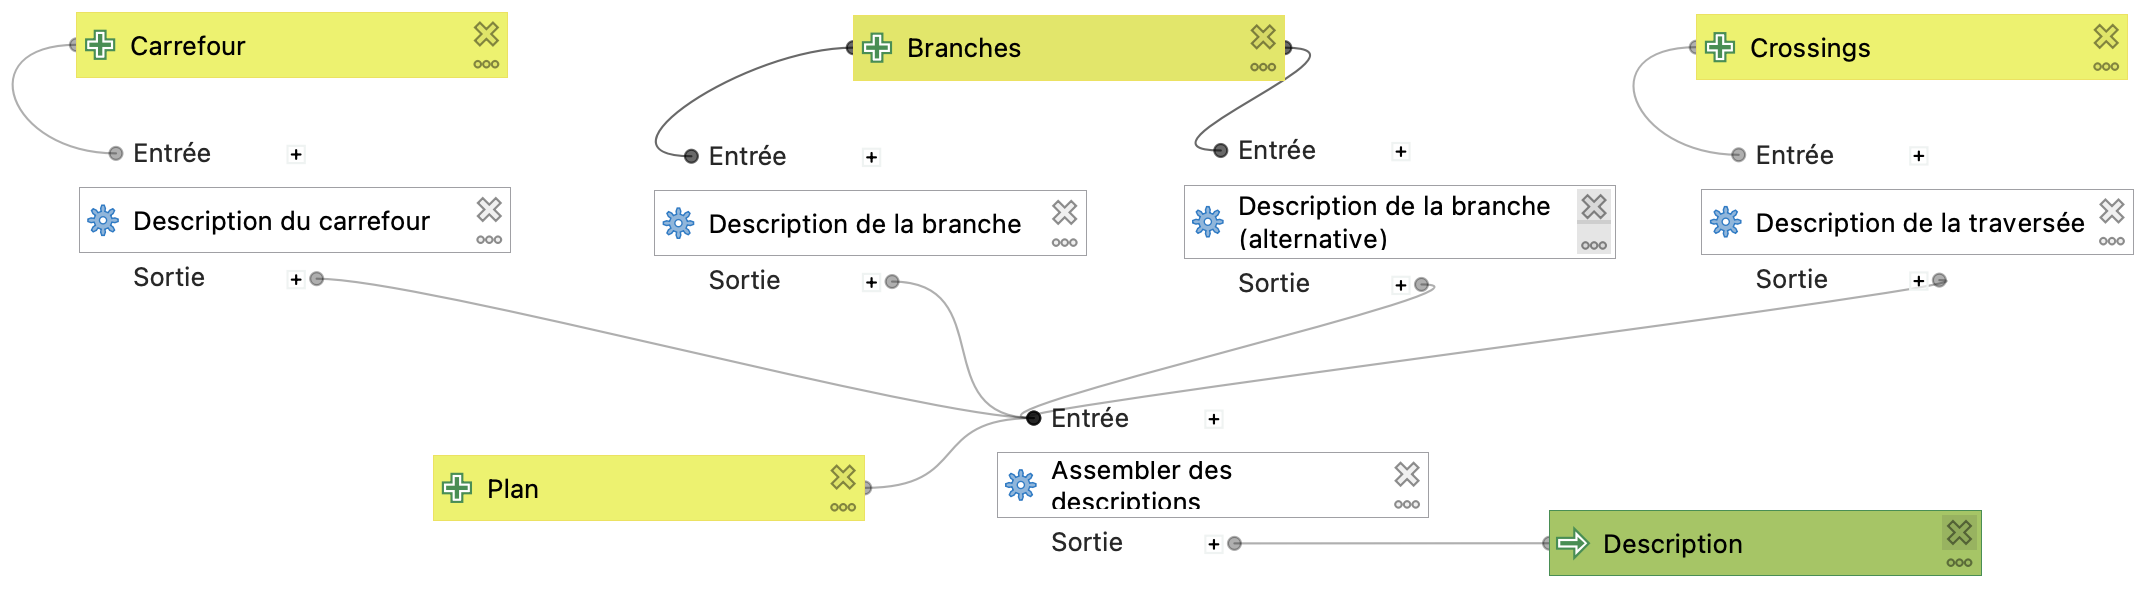
\includegraphics{images/experimentation/qgis2desc_modele_assemblage.png}}
    \caption{Le modèle graphique contient les patrons de plusieurs couches. On remarque également plusieurs patrons pour une même couche. Ceux-ci pourront être sélectionnés à l'aide des métadonnées lors de l'étape d'assemblage pour personnaliser la description.}
    \label{fig:experimentation_qgis2desc_modele_assemblage}
\end{figure}

\subsection{Utilisation des outils pour générer une description}

Les outils en place, l'utilisateur final (l'\gls{ia}) va pouvoir générer des descriptions sur plusieurs territoires. Pour cela il doit suivre les étapes suivantes:

\begin{enumerate}
    \item Utiliser crmodel pour obtenir les données intrinsèques du carrefour, les données piétonnes, et les attributs d'accessibilité. Comme évoqué précédemment, le géomaticien peut avoir préparé une boîte à outil pour l'utiliser de manière graphique.
    \item Exécuter le premier traitement préparé le géomaticien pour transformer les données  de crmodel en couche prêtes pour la description (figure \ref{fig:experimentation_chaine_donnees_qgis}).
    \item Exécuter le second traitement pour obtenir la description finale. Il est possible de personnaliser le résultat en sélectionnant les patrons préparés, et en ajustant la présence et la forme des parties. 
\end{enumerate}

L'intégralité du processus réalisé par l'utilisateur final est illustré en figure \ref{fig:experimentation_processus_realisation_utilisateur}.

\begin{figure}[ht]
    \centering
    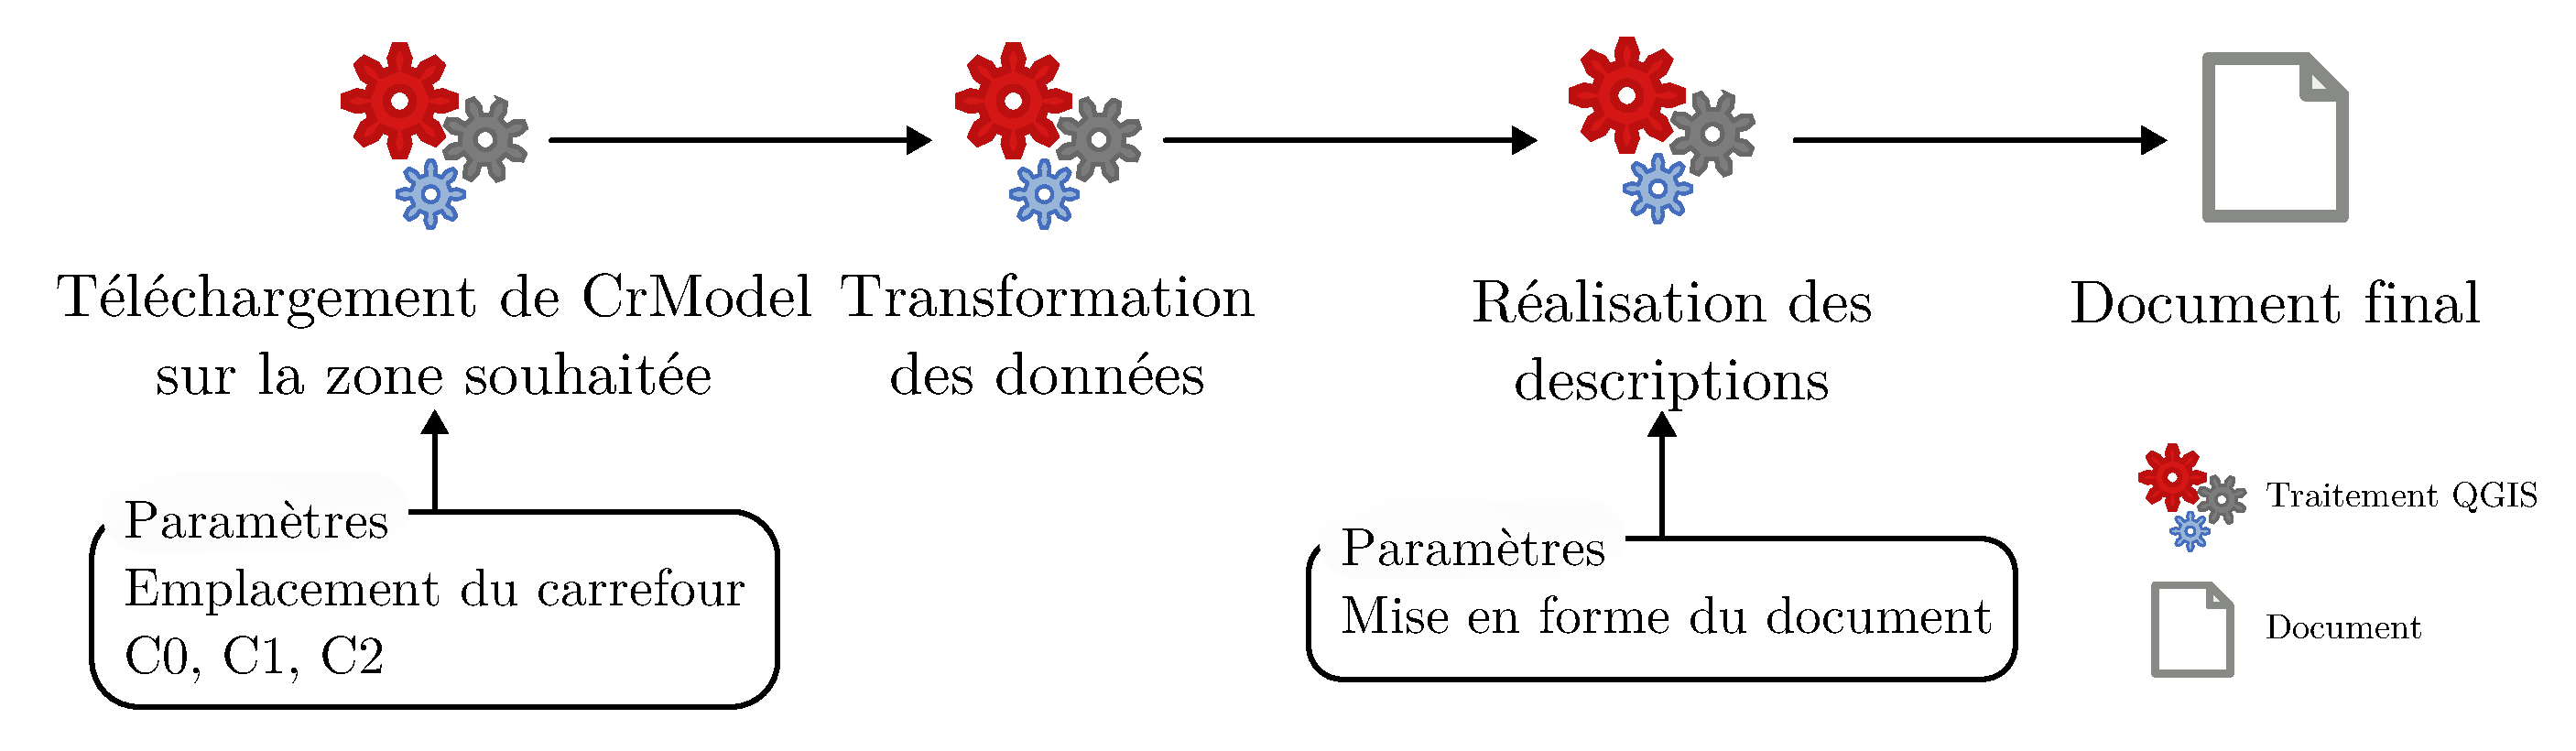
\includegraphics[width=\textwidth]{images/experimentation/pipeline_utilisateur.pdf}
    \caption{L'exécution de la chaîne complète est simplifiée par les outils réalisés en amont par le géomaticien. Les complexités des traitements de données et de la réalisation du texte sont masquées derrière des boîtes à outils dont la prise en main est facilitée.}
    \label{fig:experimentation_processus_realisation_utilisateur}
\end{figure}

\subsection{Des interfaces pour accéder aux descriptions}

% CrWeb

En parallèle des outils implémentés sous QGIS, nous avons proposé une seconde interface dans un environnement web qui imlémente le plan de description esquissé en figure \ref{fig:experimentation_plan_description}. Les traitements sont réalisés intégralement côté serveur. Lors du clic sur un carrefour, la position est envoyé au serveur qui télécharge les données \gls{osm} autour du point, segmente le carrefour le plus proche avec crseg, exécute crmodel, et réalise la description en Python de la même manière que sous QGIS. Le serveur renvoie alors au client le GeoJSON du carrefour pour afficher le résultat de la segmentation, ainsi que la description. Il est également possible côté client de personnaliser les paramètres de crseg pour moduler la segmentation du carrefour. Une capture d'écran de l'outil est présentée en figure \ref{fig:experimentation_crweb}. Par ailleurs, l'outil est accessible en ligne\footnote{https://carrefour.anatidaepho.be} et son code source l'est également\footnote{https://github.com/jeremyk6/crweb}.

\newpar{}

% Le Pigeon Nelson

Par ailleurs, le serveur permet également de renvoyer les données au format attendu par l'application "Le Pigeon Nelson". Le Pigeon Nelson est une application libre pour smartphone\footnote{https://github.com/Le-Pigeon-Nelson/le-pigeon-nelson} qui permet de jouer un son relatif à la position de l'utilisateur et aux valeurs des capteurs du téléphone. Il fonctionne en mode client-serveur et la majorité de la logique se trouve côté serveur (se référer à la documentation pour plus de détails). Lors d'une requête vers le serveur CrWeb, l'application envoie sa position GPS. Le pipeline tel que décrit précédemment est alors exécuté sur la position envoyée avec les paramètres par défaut de crseg, et le serveur renvoie un fichier JSON adapté contenant le texte généré pour le carrefour le plus proche. Ce JSON est interprété par l'application, qui lit la description obtenue par synthèse vocale. Une capture de l'application en cours d'utilisation est présentée en figure \ref{fig:experimentation_pigeonnelson}.

\begin{figure}[ht]
    \centering
    \begin{subfigure}[t]{.49\linewidth}
        \centering
        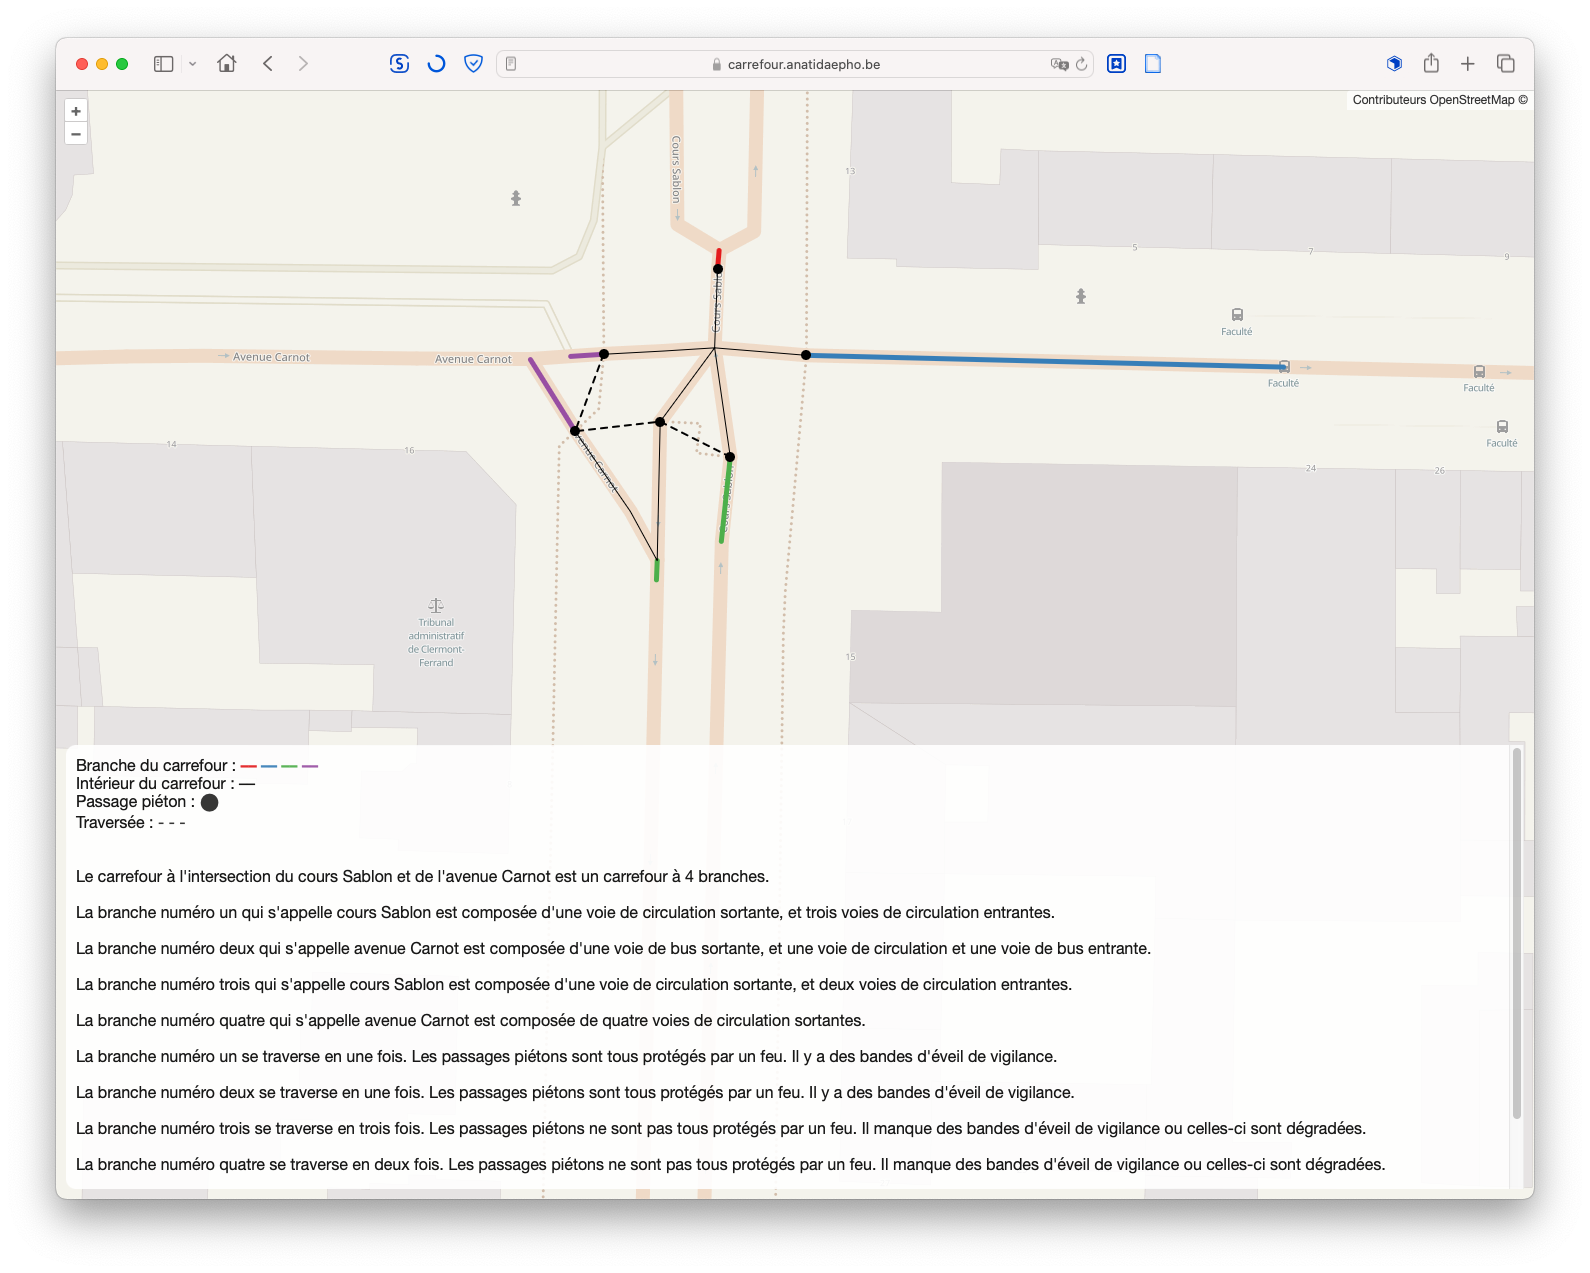
\includegraphics[width=\textwidth]{images/experimentation/crweb.png}
        \caption{CrWeb permet d'afficher la segmentation du carrefour et le résultat de la description pour un patron figé.}
        \label{fig:experimentation_crweb}
    \end{subfigure}
    \begin{subfigure}[t]{.49\linewidth}
        \centering
        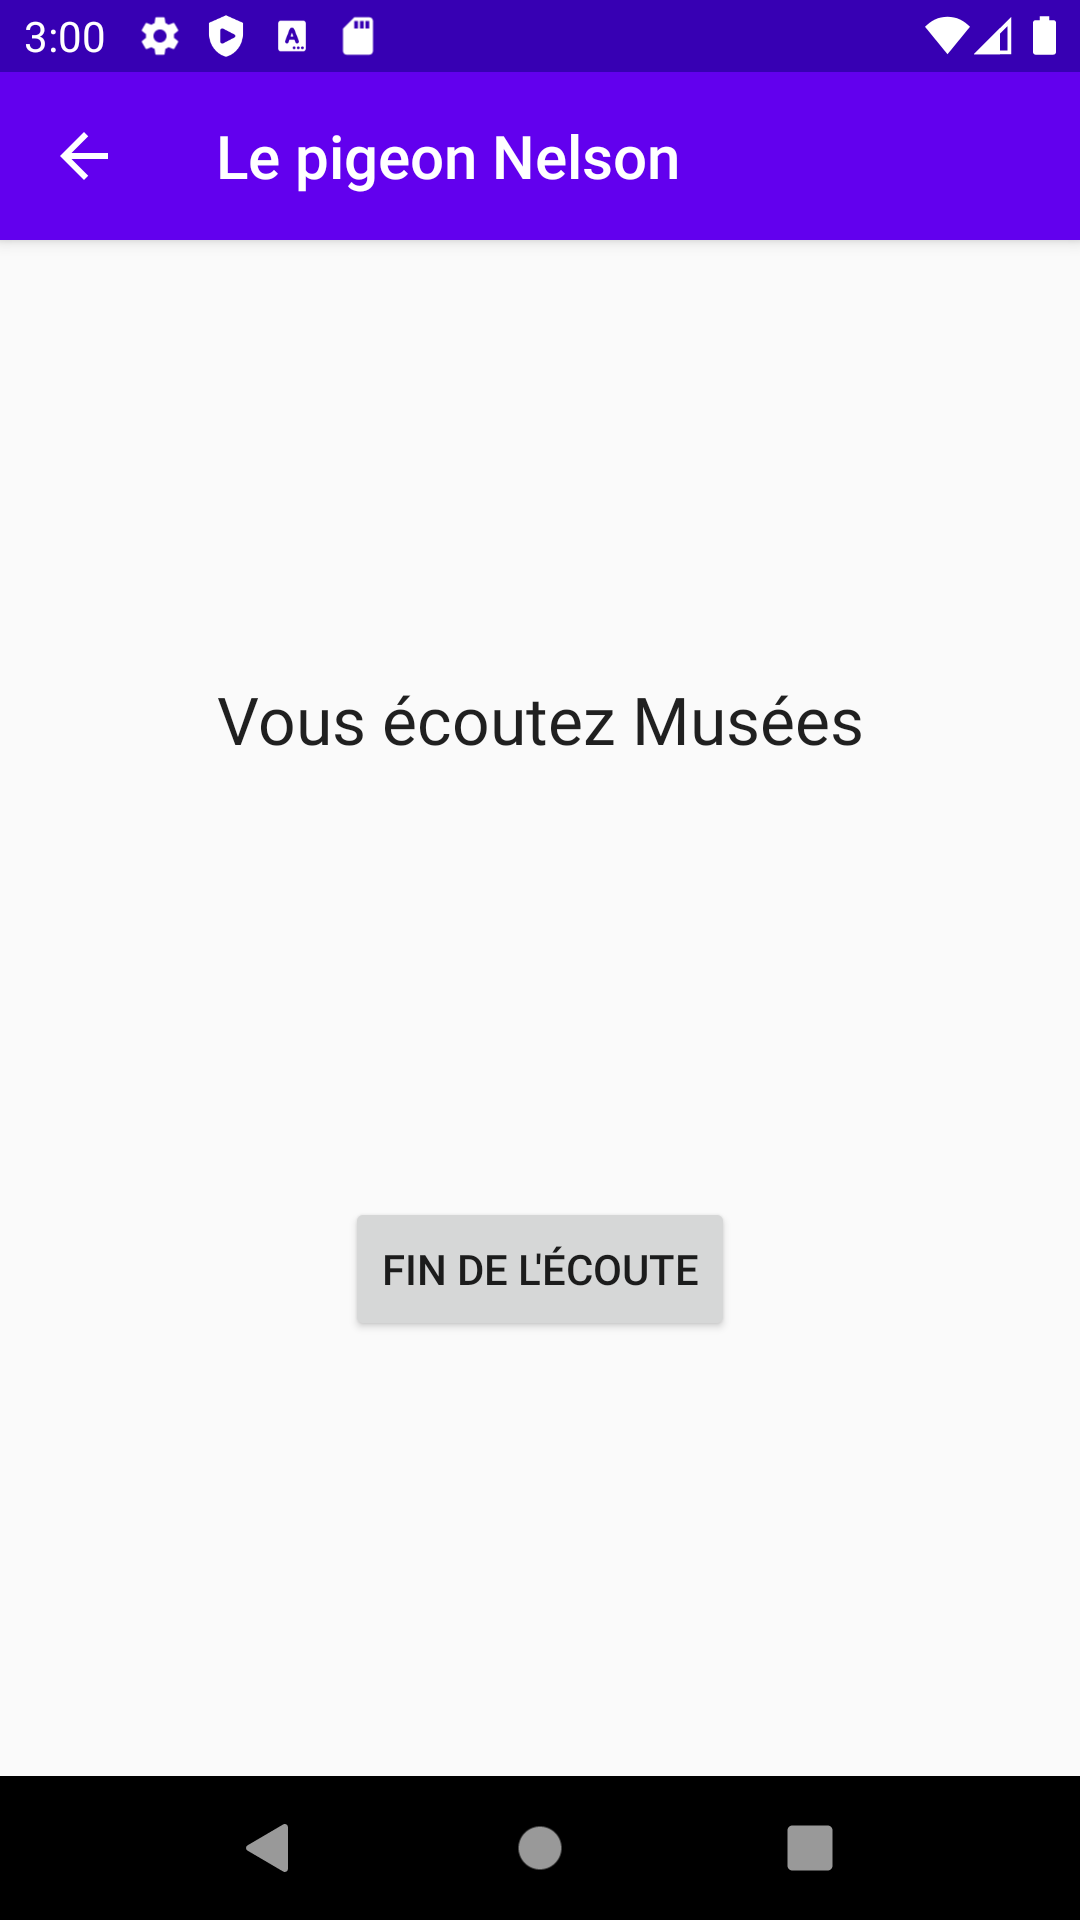
\includegraphics[width=0.4\textwidth]{images/experimentation/pigeonnelson.png}
        \caption{L'application lors de l'échange avec le serveur n'affiche aucune information. Ici, le son joué correspond au texte affiché par la figure de gauche.}
        \label{fig:experimentation_pigeonnelson}
    \end{subfigure}
    \caption{Deux exemples d'interfaces permettant d'afficher ou d'écouter les descriptions générées à l'aide des outils présentés.}
    \label{fig:experimentation_crweb_pigeon}
\end{figure}

\section{Des descriptions textuelles intégrées à une carte tactile}

Le projet ACTIVmap, dans lequel s'inscrit cette thèse, est porté par trois acteurs: le \gls{limos}, l'\gls{ign} et l'\gls{irit}. La collaboration entre ces trois entités s'est cristallisée sous la forme de preuves de concepts dont l'objectif est de présenter une chaîne partant de la donnée pour réaliser une carte audiotactile. Dans cette partie, nous présentons deux preuves de concept réalisées dans ce cadre.

\subsection{Preuve de concept 1: réaliser une carte audiotactile}

\label{sec:experimentation_poc1}

\gls{deri} \missref{} est une application développée au sein de l'\gls{irit}. Elle permet de transformer une tablette tactile en support tactile interactif. Son fonctionnement est le suivant: au sein de l'application est ouvert un fichier spécifique qui définit sur l'écran des interacteurs qui à l'appui déclenchent un son enregistré ou synthétisé. Plusieurs types d'appui sont pris en compte (simple appui, double appui), et il est possible sur un interacteur de déclencher des sons différents selon le type d'appui. Un document tactile correspondant au fichier et imprimé sur papier thermogonflé est posé sur l'écran et maintenu par la coque. L'épaisseur du papier permet aux interactions d'être détectée par l'écran tactile et de jouer les sons déclenchés par l'utilisateur lors de l'appui sur un interacteur. La figure \ref{fig:experimentation_exemple_deri} présente le dispositif.

\begin{figure}
    \centering
    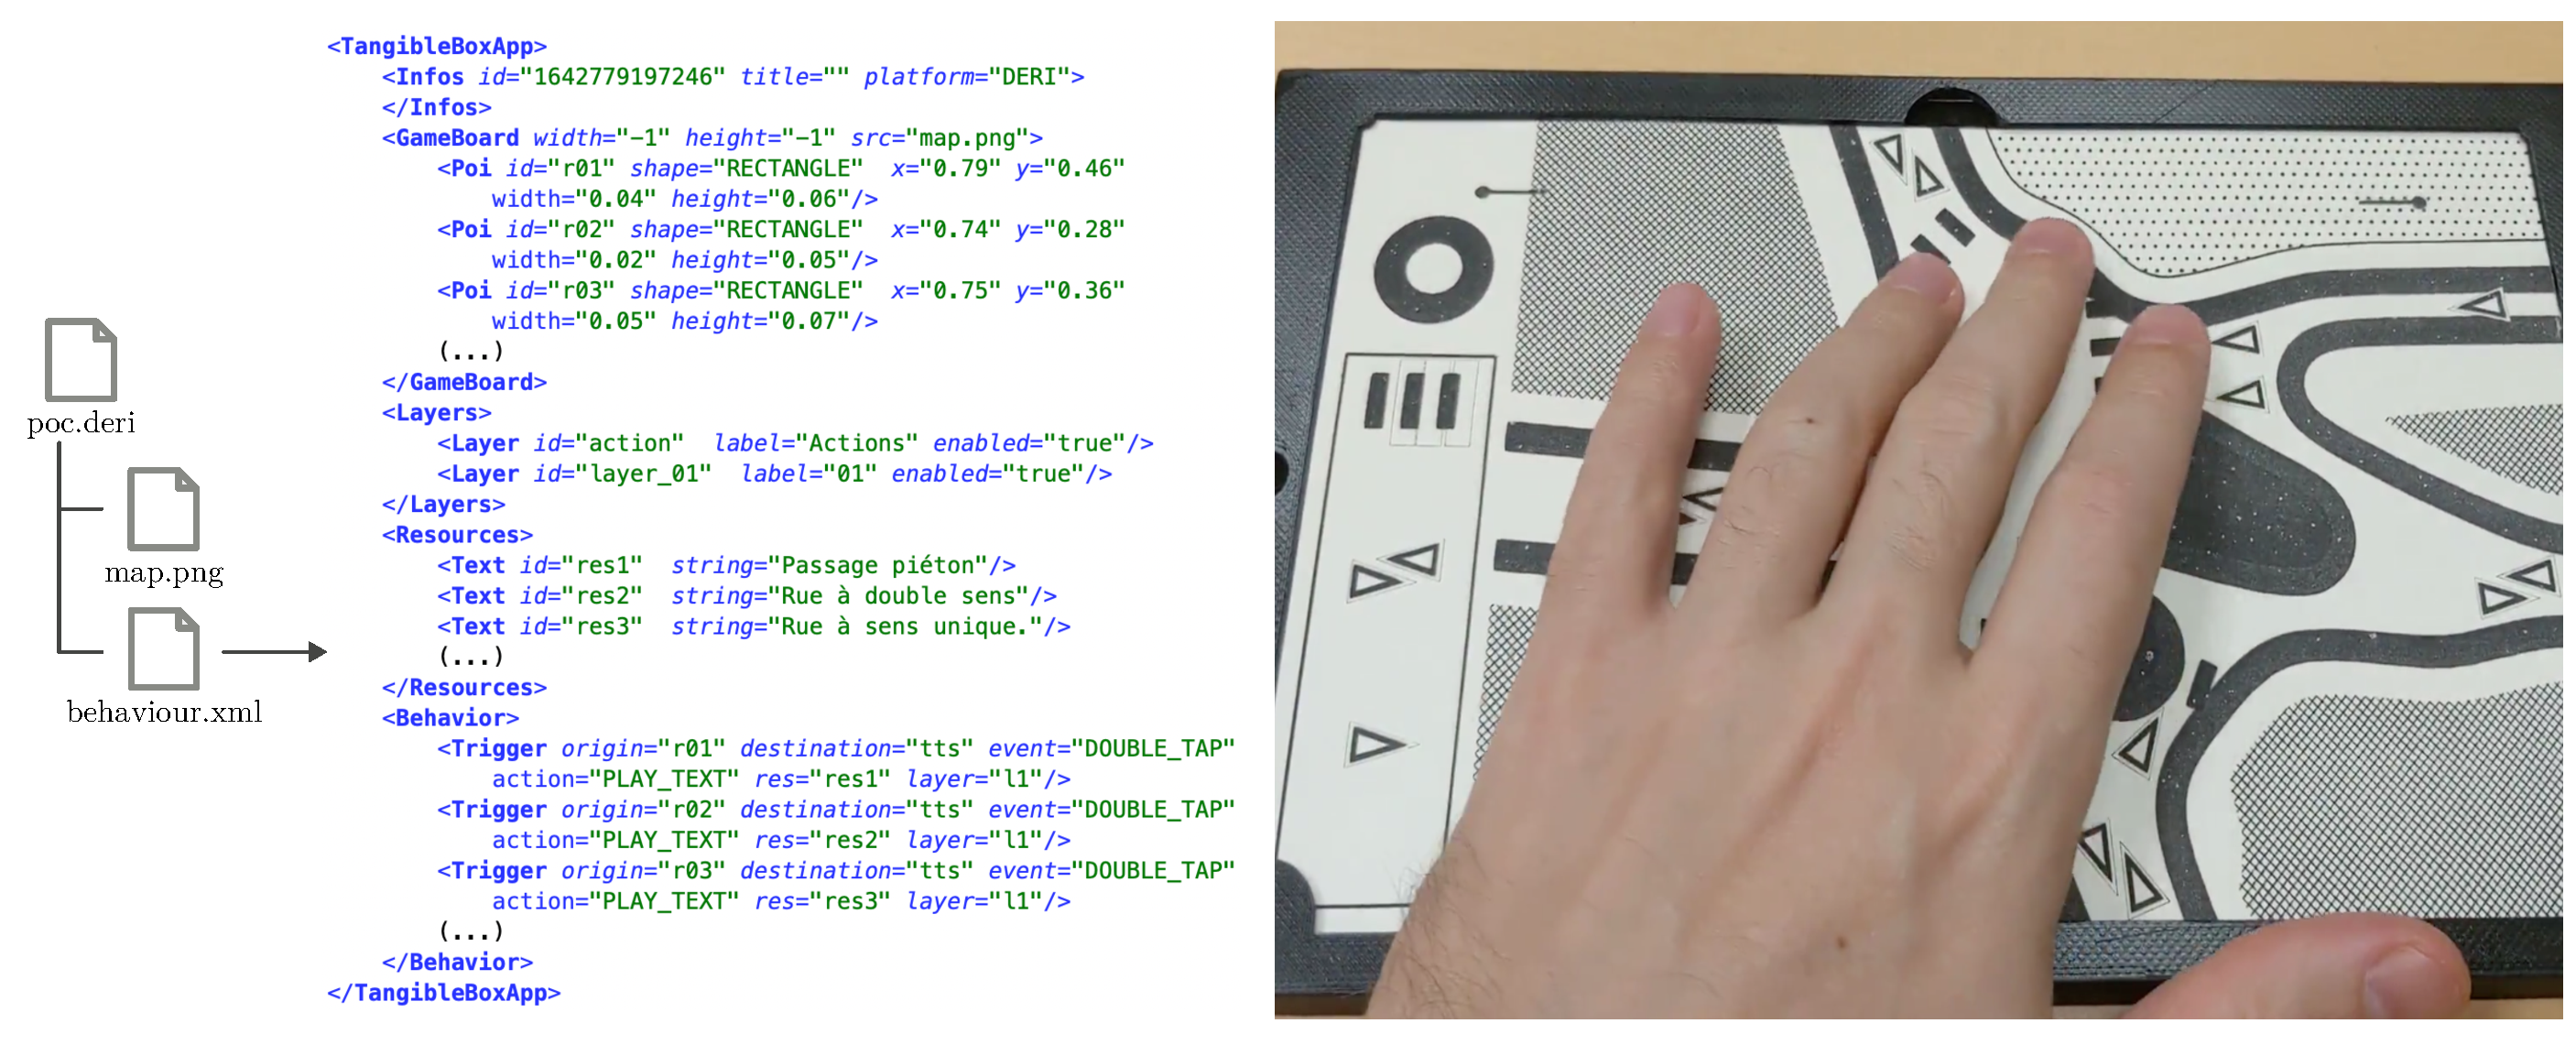
\includegraphics[width=\textwidth]{images/experimentation/exemple_deri.pdf}
    \caption{À gauche, contenu d'un fichier .deri et extrait du fichier XML d'interaction pour la légende de la carte de droite. On remarque que sont définis séparément les interacteurs (Poi) et les textes à jouer (Text), liés ensemble par une interaction (Trigger). À droite, une tablette \gls{deri} assemblée et en cours d'utilisation. Source: preuve de concept ACTIVmap.}
    \label{fig:experimentation_exemple_deri}
\end{figure}

\gls{deri} peut être utilisé pour réaliser toute sorte de documents audiotactiles, dont des cartes pour prendre connaissance d'un lieu \missref{}. En revanche, ces réalisations à l'instar de celles des \gls{ia} sont aujourd'hui manuelles. L'objectif de cette expérimentation est de permettre la génération d'une carte audiotactile de carrefour sous la forme d'un fichier \gls{deri}. La chaîne permettant d'obtenir le document final combine les description développées au \gls{limos} et les cartes tactiles développées à l'\gls{ign}.

\subsubsection{Assembler la carte et les descriptions}

Dans la partie \ref{sec:implementation_segmentation}, nous avons présenté un cadre et les outils permettant de proposer une description textuelle de toute donnée géographique. Par ailleurs, nous avons proposé des outils permettant à partir des données \gls{osm} d'obtenir des informations intrinsèques au carrefour comme la délimitation des branches. Tous ces outils peuvent être intégrés au \gls{sig} QGIS pour décrire textuellement un carrefour. Les travaux de \citet{Jiang2023} s'intéressent à la génération de cartes tactiles à l'échelle du carrefour, en partant également des données d'\gls{osm}. Les processus transforment les géométries et stylisent les données pour les adapter aux contraintes de lisibilité d'une carte tactile imprimée sur du papier thermogonflé. Ces processus s'intègrent également à QGIS.

\newpar{}

La réalisation d'une carte audiotactile à partir des travaux cités soulève les questions suivantes:

\begin{itemize}
    \item \textbf{Quels éléments décrire ?} \\
    Le choix des éléments à décrire dépendra de la taille et de l'usage de la carte (voir les exemples présentés en partie \todo{}). Les outils présentés en partie \ref{sec:implementation_segmentation}, en particulier les traitements intégrés à QGIS2Desc, permettent d'étendre les possibilités de description à des données non-intégrées à crmodel aujourd'hui. Outre l'accessibilité, il est alors possible de décrire d'autres points d'intérêts pouvant servir de repère tels que les commerces ou les arrêts de bus.
    \item \textbf{Où et comment placer les interacteurs pour maintenir la lisibilité de la carte ?} \\
    Les sons joués par \gls{deri} sont déclenchés par des interacteurs. Les interacteurs sont intégrés à une couche indépendante des données géographiques à décrire. Par exemple, l'interacteur permettant de décrire un passage piéton peut être placé à côté de celui-ci et non-pas sur le symbole représentant le passage piéton pour ne pas gêner sa lisibilité. Une grande densité d'interacteurs peut également poser des problèmes de lisibilité, et il est alors souhaitable de les fusionner. Le placement des interacteur est un problème qui n'a aujourd'hui pas encore été abordé et fait partie des perspectives évoquées par \cite{Jiang2023}. Leur placement est ici défini à la main.
    \item \textbf{Comment définir le texte d'un interacteur ?} \\
    En partant des mêmes données pour la carte et pour le texte, il existe un identifiant commun issu d'\gls{osm} pour chaque entité  permettant d'effectuer une correspondance automatique. Cependant, certaines descriptions n'ont pas d'accroche sous la forme d'un objet issu d'\gls{osm}. Il peut s'agir par exemple de la description générale du carrefour, ou des description de branches. L'identifiant permettant de faire la correspondance avec le texte doit alors être décidé en amont pour être commun aux deux données.
\end{itemize}

\newpar{}

Une illustration de la chaîne de traitement partant des données jusqu'au lien entre le texte généré et la carte tactile est présentée en figure \ref{fig:experimentation_lien_carte_texte}.

\begin{figure}[ht]
    \centering
    
\includegraphics{images/placeholder.jpg}
    \caption{Cette chaîne présente la méthode choisie pour définir le texte des interacteurs de la carte tactile en fonction des objets qu'ils représentent. Ce lien est fait en utilisant l'idenfiant \gls{osm} commun au texte et à la carte.}
    \label{fig:experimentation_lien_carte_texte}
\end{figure}

\subsubsection{Générer un fichier \gls{deri}}

À partir du fichier du fichier des interacteurs décrits et de la carte, il est possible de générer un fichier \gls{deri}, mais une transformation de la forme et des coordonnées doit être effectuée. Un fichier \gls{deri} correspond à un fichier zip contenant la carte dans un format image pour un affichage à l'écran (pour tester les interactions) et un fichier XML définissant les interactions. Ce dernier est séparé en trois parties principales: définition de la position et de la forme des interacteurs, définition des ressources (textes à lire ou fichiers audio), et définition pour chaque interacteur de la ressource jouée pour une interaction donnée (simple appui, double appui, etc.) (voir figure \ref{fig:experimentation_exemple_deri}). 

\newpar{}

\gls{deri} étant un système permettant la réalisation de tout document tactile, donc pas spécialement des cartes, la position et la forme des interacteurs est exprimée en pourcentage de taille d'écran, avec une origine en haut à gauche. Pour calculer la position dans ce format ($x_{deri}$ et $y_{deri}$) de chaque interacteur, il est donc nécessaire de connaître la position de chaque interacteur ($x$ et $y$) et l'étendue de la carte ($x_{min}$, $x_{max}$, $y_{min}$ et $y_{max}$):

\newpar{}

$x_{deri} = \frac{x - x_{min}}{x_{max} - x_{min}}$

$y_{deri} = \frac{y - y_{min}}{y_{max} - y_{min}}$

\newpar{}

Le processus de transformation, à l'instar des précédents, peut être automatisé dans un \gls{sig} comme QGIS pour obtenir le document final.

\subsubsection{Exemples de cartes audiotactiles générées}

Les méthodes présentées dans cette partie ont été appliquées à la génération de cartes audiotactiles de différentes tailles et répondant à différents usages. La figure \ref{fig:experimentation_exemples_cartes_audiotactiles} présente quelques exemples de résultats.

\begin{figure}[ht]
    \centering
    \begin{subfigure}[t]{.49\linewidth}
        \centering
        
\includegraphics[width=\textwidth]{images/placeholder.jpg}
    \end{subfigure}
    \begin{subfigure}[t]{.49\linewidth}
        \centering
        
\includegraphics[width=\textwidth]{images/placeholder.jpg}
    \end{subfigure}
    \caption{Deux cartes audiotactiles réalisées par Markie Jiang \cite{jiang:tel-04500971} dans le cadre du projet. La différence de taille entre les deux carte (A4 à gauche, A5 à droite) s'explique par la différence d'usage. La première est pensée pour être utilisée chez soi ou en séance de locomotion. La seconde est plutôt prévue pour un usage sur site.}
    \label{fig:experimentation_exemples_cartes_audiotactiles}
\end{figure}

\subsection{Preuve de concept 2: interactions à partir de données graphe}

% Inspiré des interactions avec un téléphone

Dans l'expérimentation précédente, nous avons proposé les méthodes permettant de générer une carte audiotactile pour \gls{deri} à partir d'une carte et de données géographiques décrites. Dans sa version actuelle, \gls{deri} permet de définir un son par interaction et par interacteur. Cela correspond bien à un usage exploratoire de la carte, mais cela limite la quantité d'information que l'on peut faire figurer. Par exemple, en fonction de l'échelle de la carte il n'est pas possible de faire figurer tous les services (commerces, banques, bureaux de postes, etc) d'une branche pour des contraintes de lisibilité, la densité des interacteurs nécessaires pouvant être trop importante ou le texte trop long si présent sur un seul interacteur. Par ailleurs, il pourrait être souhaitable de décrire la branche au-delà de ce que la carte affiche. Pour répondre à cette problématique dont l'objectif est de réfléchir à de nouveaux usages, l'\gls{irit} propose de faire figurer des informations multiples sur un seul interacteur sous la forme d'un graphe de texte navigable par glissement du doigt, à l'instar de la navigation actuellement implémentée sur les smartphones \missref{}. Nous avons proposé ensemble une nouvelle version du format de fichier \gls{deri} permettant d'implémenter un graphe de texte au sein d'un unique interacteur. Le fonctionnement de ce nouveau format et son application possible à la navigation virtuelle au sein d'une branche sont détaillées dans cette partie.

\subsubsection{\gls{deri} 2: un nouveau format pour naviguer dans un graphe de textes}

À l'instar de la première version, un fichier \gls{deri} 2 est également un fichier zip contenant une image du document et un fichier d'interaction. Ce dernier est maintenant au format JSON et comprend les mêmes sections que précédemment. La différence majeure se situe dans la capacité des ressources à être liées à d'autres ressources en fonction d'une nouvelle interaction. En déclenchant depuis un interacteur une ressource donnée, un curseur virtuel est placé sur cette ressource. Une nouvelle interaction réalisée sur le même interacteur pourra déplacer ce curseur vers une nouvelle ressource. Les ressources forment ainsi un graphe au sein duquel il est possible de naviguer par interaction. Outre les appuis, les glisser dans les quatres directions ont été introduits pour permettre la navigation dans le graphe. La figure \ref{fig:experimentation_deri2_exemple} illustre le fonctionnement de ce nouveau format.

\begin{figure}[ht]
    \centering
    
\includegraphics{images/placeholder.jpg}
    \caption{Le fichier JSON d’interaction décrit un graphe de texte navigable par interaction. La carte de droite illustre le passage d'un texte à un autre selon l'interaction réalisée.}
    \label{fig:experimentation_deri2_exemple}
\end{figure}

Cette nouvelle représentation sous forme de graphe permet de spatialiser les descriptions, avec une notion d'avant et d'après. Dans cette expérimentation, nous avons choisi d'appliquer ce nouveau format  à la description interactive d'une branche, et en particulier de ses commerces et services. L'objectif est ici de pouvoir naviguer depuis le début de la branche de commerce en commerce, et d'entrer virtuellement à l'interieur de ceux-ci pour obtenir des informations supplémentaires sur chacun d'eux. Une illustration des textes souhaités est présentée en figure \ref{fig:experimentation_deri2_template}.

\newpar{}

\begin{figure}[ht]
    \centering
    
\includegraphics{images/placeholder.jpg}
    \caption{Pour chaque type d'objet décrit, un patron textuel spécifique est appliqué.}
    \label{fig:experimentation_deri2_template}
\end{figure}

\subsubsection{Traitement des données pour la génération du graphe}

À l'instar de la première preuve de concept, les données mobilisées seront issues de crmodel pour les informations du carrefour, complétées d'\gls{osm} pour les commerces. Pour réaliser ces textes, il est nécessaire de concevoir un graphe par branche. Ce graphe sera réalisé de la manière suivante:

\begin{itemize}
    \item Pour chaque branche, on estime quels commerces se situent sur son trottoir de droite et sur son trottoir de gauche.
    \item Un graphe de proximité des commerces par trottoir est réalisé. Chaque nœud permettra d'indiquer le nom et l'adresse du commerce.
    \item Un nœud supplémentaire est ajouté par commerce. Il est relié au nœud du commerce concerné et permet d'indiquer des informations supplémentaires telles que les horaires d'ouverture et les services proposés.
    \item Aux graphe de proximité des commerces sont insérés les nœuds des passages piétons présents sur la branches. Leurs deux extrémités permettent de naviguer d'un trottoir à l'autre.
\end{itemize}

\newpar{}

La construction de ce graphe pour une branche est illustrée en figure \ref{fig:experimentation_deri2_construction_graphe}. Elle peut être automatisée sous QGIS et présentée sous la forme d'une boîte de traitement.

\begin{figure}[ht]
    \centering
    
\includegraphics{images/placeholder.jpg}
    \caption{La construction du graphe d'interaction pour une branche d'un carrefour s'effectue en plusieurs étapes.}
    \label{fig:experimentation_deri2_construction_graphe}
\end{figure}

L'implémentation des patrons textuels est ensuite réalisée avec QGIS2Desc pour chaque type de nœud du graphe (commerce, passage piéton, etc).

\subsubsection{Construction du fichier \gls{deri} 2}

Le fichier 

\todo{}

\subsubsection{Exemple de carte audiotactile générée}

\todo{}

\section{Le carrefour dont vous êtes le héros  : naviguer dans une description égocentrée}

Les outils de la partie précédente ont été présentés sur une chaîne de traitement permettant la réalisation d'une description exocentrée de carrefour sous la forme d'un texte figé. L'étape d'assemblage présentée génère un document HTML, mais il est possible de l'étendre pour générer d'autres types de documents balisés. Dans cette partie, nous présentons une expérimentation permettant de décrire textuellement le carrefour en apportant une dimension interactive à la navigation virtuelle au sein de celui-ci. Pour cela, le carrefour sera modélisé sous la forme d'un graphe.

\todo{}

\subsection{Texte souhaité et forme des données}

Au contraire de la description exocentrée qui présente l'intégralité du carrefour au sein d'un texte, la description egocentrée 

\todo{}

\section{Conclusion du chapitre}

